\documentclass{article}
\usepackage{graphicx}
\usepackage{soul} % needed
\usepackage[utf8]{inputenc}
\usepackage{listings}
\usepackage{hyperref}
\usepackage{chemformula}
\usepackage{amssymb}
\usepackage{amsmath}
\usepackage{soul}
\title{Chemistry Assignment 3.5}
\author{Wenqi Guo}
\date{December 2022}

\begin{document}

\maketitle
\newcommand{\tab}{\;\;\;\;\;}
\begin{large}


\section{Calculation Problem}
\subsection{Find the concentration of all species in an aqueous solution containing 0.10 M \ch{CH3COONa}}
Based on the question, we can get the following reactions
\begin{equation}
% [\ch{CH3COO-}] + [\ch{Na}] = [\ch{CH3COONa}]
% \end{equation}
\ch{CH3COO-} + \ch{Na} \leftrightarrow \ch{CH3COONa}
\end{equation}
\begin{equation}
\ch{CH3COO-} + \ch{H+} \leftrightarrow \ch{CH3COOH}
\end{equation}
\begin{equation}
\ch{H+} + \ch{OH-} \leftrightarrow \ch{H2O}
\end{equation}
And based on the charge balance, we can get
\begin{equation}
[\ch{CH3COO-}] + [\ch{OH-}] = [\ch{Na+}] + [\ch{H+}]
\end{equation}
And based on the mass balance, we can get
\begin{equation}
[\ch{Na+}] = 0.10M
\end{equation}
\begin{equation}
[\ch{CH3COOH}] + [\ch{CH3COO-}] = 0.10M
\end{equation}
% We find the $K_{sp}$ of the \ch{CH3COOH} and \ch{CH3COONa}
\text{For reaction (3)}
\begin{equation}
[\ch{H+}][\ch{OH-}]=10^{-14}
\end{equation}
For reaction (2)

\begin{equation}
K_a = \frac{[\ch{H+}][\ch{CH3COO-}]}{[\ch{CH3COOH}]}  = 1.8 \times 10^{-5}
\end{equation}
$\because$ All \ch{CH3COONa} is in dissolved\\$\therefore$ Reaction (1) is not in equilibrium.

We have 4 unknowns: \ch{H+}, \ch{OH-}, \ch{CH3COO-}, and \ch{CH3COOH}. 

Combining (4) and (5), we get
\begin{equation}
[\ch{CH3COO-}] + [\ch{OH-}] = 0.10M + [\ch{H+}]
\end{equation}
% And we have 4 equations: (8), (7), (6), and (9).
% Set $a=\ch{H+}, b=\ch{OH-}, c=\ch{CH3COO-}, \text{and} d=\ch{CH3COOH}$.
From (6) we can get 
\begin{equation}
[\ch{CH3COO-}] = 0.10M - [\ch{CH3COOH}]
\end{equation}
Combine (9) and (10), and we got
\begin{equation}
    0.10M - [\ch{CH3COOH}] + [\ch{OH-}] = 0.10M + [\ch{H+}]
\end{equation}
Then we got
\begin{equation}
     [\ch{OH-}] - [\ch{CH3COOH}] = [\ch{H+}]
\end{equation}
% \begin{equation}
%      \frac{- [\ch{CH3COOH}]}{[\ch{H+}]} + \frac{[\ch{OH-}]}{[\ch{H+}]} = 1
% \end{equation}
% \begin{equation}
%      \frac{- [\ch{CH3COOH}]}{[\ch{H+}]} + \frac{[\ch{OH-}]}{[\ch{H+}]} = 1
% \end{equation}
$\because$ The solution has a pH greater then 7.0\\$\therefore$ we can assume [\ch{H+}] is small and can be ignored. 
Thus, we can make (12) as
\begin{equation}
    [\ch{OH-}] - [\ch{CH3COOH}] \approx 0
\end{equation}
\begin{equation}
    [\ch{OH-}] \approx [\ch{CH3COOH}]
\end{equation}
Replace [\ch{CH3COOH}] with [\ch{OH-}] in (8), we get
\begin{equation}
\frac{[\ch{H+}][\ch{CH3COO-}]}{[\ch{OH-}]}  = 1.8 \times 10^{-5}    
\end{equation}
Based on (10), (15), and (14), we got
\begin{equation}
\frac{[\ch{H+}](0.10M-[\ch{OH-}])}{[\ch{OH-}]}  = 1.8 \times 10^{-5}    
\end{equation}
Based on (16) and (7), we can solve for [\ch{OH-}] and [\ch{H+}].
\begin{equation}
\frac{
    10^{-14} (0.1-[\ch{OH-}])
}{
[\ch{OH-}]^2
} = 1.8 \times 10^{-5}
\end{equation}
Solve this, we get $[\ch{OH-}] = 0.0000075 = 7.5 \times 10^{-6}M$\\
Plug this into (7), we got $$[\ch{H+}] = \frac{10^{-14}}{7.5 \times 10^{-6}} = 1.33333 \times 10^{-8}M$$\\
(Tried so many times and finally got a result that looks right)\\
Then based on (9), we get:
\begin{equation}
[\ch{CH3COO-}] + 7.5 \times 10^{-6}M = 0.10 M + 1.33 \times 10^{-8}M
\end{equation}
This gives us $$[\ch{CH3COO-}] = 0.10 M + 1.33333 \times 10^{-8} - 7.5 \times 10^{-6} = 0.0999925133M$$\\
Then based on (6), we get $$[\ch{CH3COOH}] = 0.1M - 0.0999925133M = 7.4867\times 10^{-6}M$$\\
$$\therefore [\ch{CH3COOH}]=7.4867\times 10^{-6}M$$
$$ [\ch{CH3COO-}]=0.0999925133M$$ $$[\ch{OH-}] = 7.5\times 10^{-6}$$
% , \text{and}  
$$[\ch{H+}] = 1.33333 \times 10^{-8}M$$
$$[\ch{Na+}] = 0.10M$$

\subsection{Find the ionic strength and activity coefficients of all relevant species}
\begin{equation}
\mu = \frac{1}{2}\sum_i c_i z_i^2
\end{equation}
Plug in our ions, we can get
\begin{equation}
\frac{    7.4867\times 10^{-6}M + 1.33333 \times 10^{-8}M + 7.5\times 10^{-6}M + 0.0999925133 + 0.1}{2}  = 0.1000037567M
%  Forgot Na+
\end{equation}
Thus, we can get 
\begin{equation}
log \gamma_{\ch{CH3COO-}} = \frac{-0.51z^2\sqrt{\mu}}{1+(\alpha \sqrt{\mu}/305)} = 
\frac{-0.51\sqrt{\mu}}{1+(450\sqrt{\mu}/305)} = -0.121269473
% -0.51(sqrt(0.1000037567))/(1+(450*sqrt(0.0500037567)/305))
\end{equation}

\begin{equation}
log \gamma_{\ch{Na+}} = \frac{-0.51z^2\sqrt{\mu}}{1+(\alpha \sqrt{\mu}/305)} = 
\frac{-0.51\sqrt{\mu}}{1+(450\sqrt{\mu}/305)} = -0.121269473
% -0.51(sqrt(0.1000037567))/(1+(450*sqrt(0.0500037567)/305))
\end{equation}

\begin{equation}
log \gamma_{\ch{OH-}} = \frac{-0.51z^2\sqrt{\mu}}{1+(\alpha \sqrt{\mu}/305)} = 
\frac{-0.51\sqrt{\mu}}{1+(350\sqrt{\mu}/305)} = -0.12834491
% -0.51(sqrt(0.1000037567))/(1+(350*sqrt(0.0500037567)/305))
\end{equation}

\begin{equation}
log \gamma_{\ch{H+}} = \frac{-0.51z^2\sqrt{\mu}}{1+(\alpha \sqrt{\mu}/305)} = 
\frac{-0.51\sqrt{\mu}}{1+(900\sqrt{\mu}/305)} = -0.0971650283
% -0.51(sqrt(0.1000037567))/(1+(900*sqrt(0.0500037567)/305))
\end{equation}

% \begin{equation}
% \gamma_{\ch{CH3COO-}} = 10^{-0.0857520772} = 0.820819986651  
% \end{equation}

% \begin{equation}
% \gamma_{\ch{Na+}} = 10^{-0.0857520772} = 0.820819986651  
% \end{equation}

% \begin{equation}
% \gamma_{\ch{OH-}} = 10^{-0.0907552608} =   0.811418189829
% \end{equation}

% \begin{equation}
% \gamma_{\ch{H+}} = 10^{-0.0687073409} =   0.85367518845
% \end{equation}

We can use these values to calculate our new K.

\textbf{I forgot to include \ch{Na+} in my ion strength, so I need to redo these. I did not update the \LaTeX 
 file but my code directly, so the following results are wrong (the equation was still right). The code provides the right result.}

\[
    K_a = \frac{\gamma_{\ch{CH3COO-}}[\ch{CH3COO-}]\gamma_{\ch{H+}}[\ch{H+}]}
    {\gamma_{\ch{CH3COOH}}[\ch{CH3COOH}]}
    
    % $$$$
    % \frac{0.820819986651 \times 0.0999925133 \times 0.85367518845\times  1.333 \times 10^{-8}}{7.4867 \times 10^{-6}} = 0.000124
\]
By the same logic, we can get K_w
% $$K_w = 0.811418189829 \times 0.85367518845 \times 7.5 \times 10^{-6} \times 1.333333 \times 10^{-8}$$
% $$=6.9268740294 \times 10^{-14}$$

\\
We then use this new $K_a$ value to calculate the new concentration to convergence. \\
I wrote a python script to do this and the code can be accessed by \url{https://colab.research.google.com/drive/1fzMQiQbMUwur1lclO73721MHHMe-8Baf?usp=sharing}

This result is from the code for the first 4 epochs:
\begin{itemize}

\item $C_H:1.3416907874315686e-09, C_{OH}:7.453282152397606e-06, C_A:0.09999254805953839, C_{HA}:7.451940461616902e-06, K_w:6.283993135113452e-15, k_a:1.1533270162412636e-05$

\item $C_H:8.513538654863563e-10, C_{OH}:7.381176488255645e-06, C_A:0.09999261967486561, C_{HA}:7.380325134392907e-06, K_w:3.948857186708355e-15, k_a:7.389317950156082e-06$

\item $C_H:5.40198986124516e-10, C_{OH}:7.310004809594631e-06, C_A:0.0999926905353894, C_{HA}:7.309464610610883e-06, K_w:2.4814594127897206e-15, k_a:4.73410910046989e-06$

\item $C_H:3.4275866335143117e-10, C_{OH}:7.239669417911911e-06, C_A:0.09999276067334076, C_{HA}:7.239326659247425e-06, K_w:1.559347641898234e-15, k_a:3.032917923524512e-06$
\end{itemize}

(The result from the first epoch is different than what I did above because the precision of my calculator was not enough)

The core code logic is this:\\
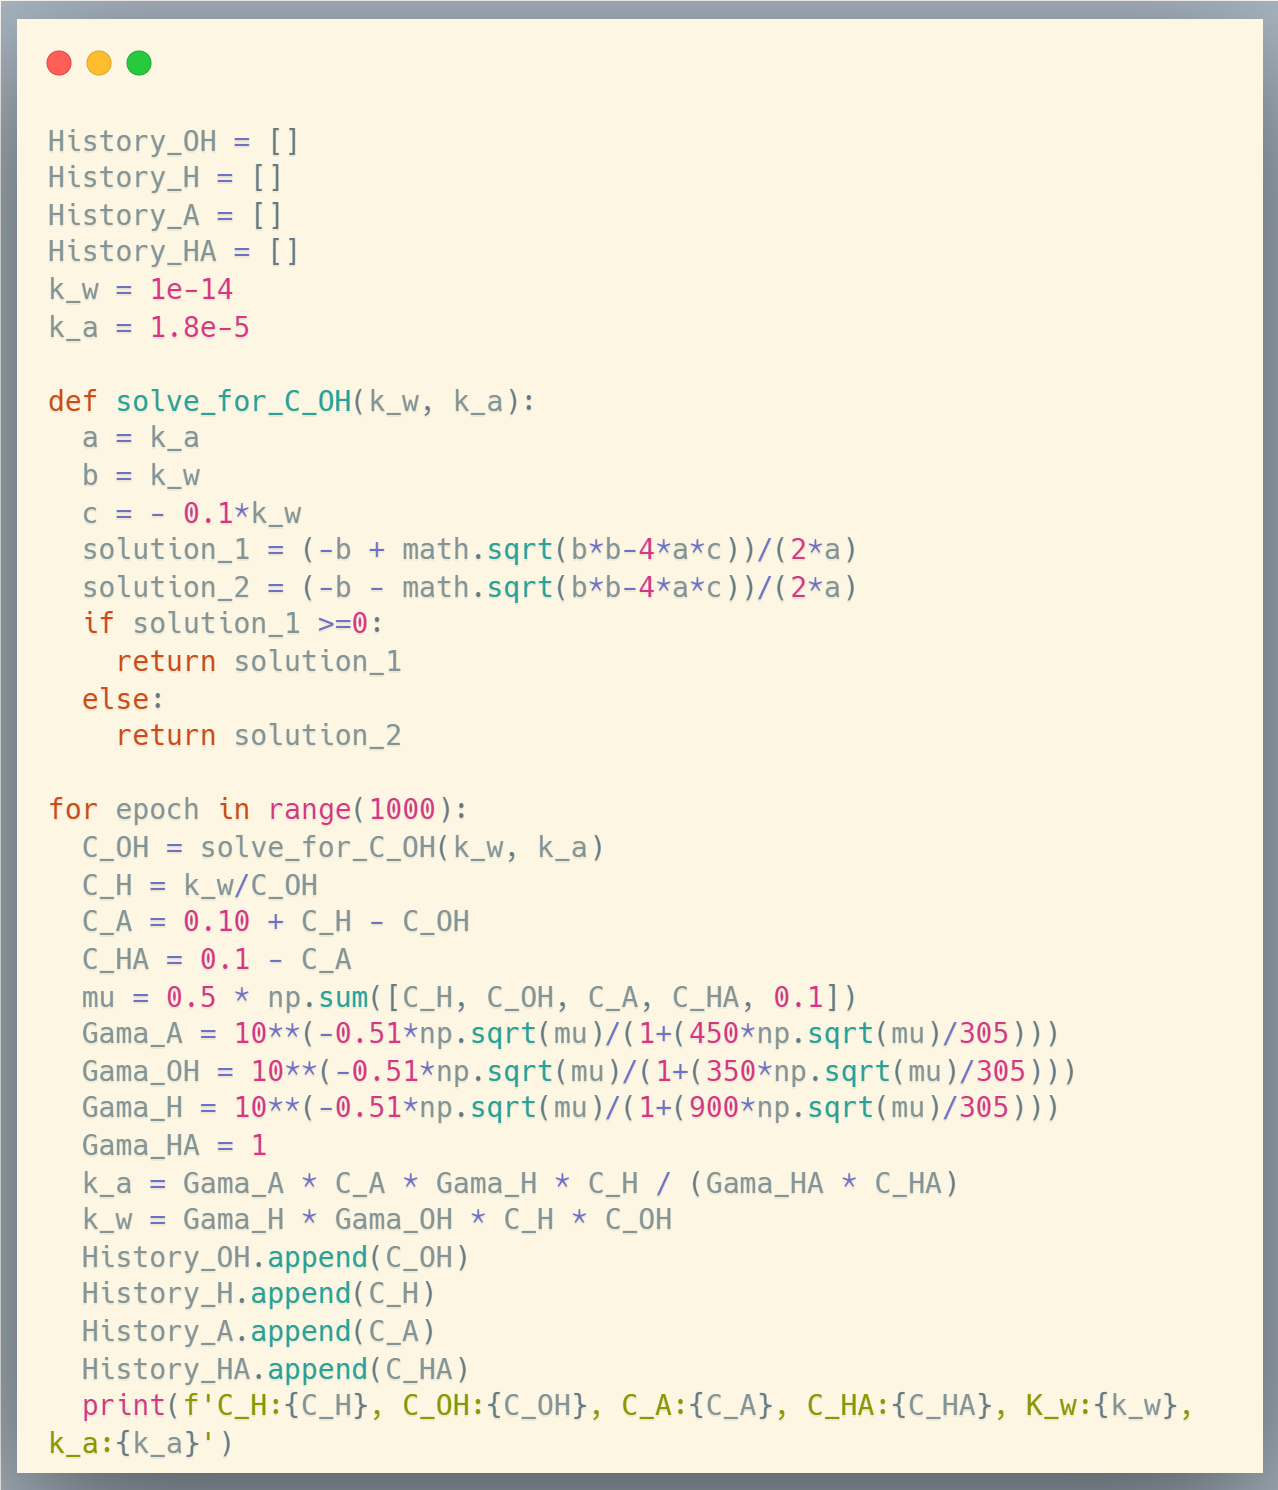
\includegraphics[width=15cm]{carbon.png}
And the converging process is shown below: (next page)\\
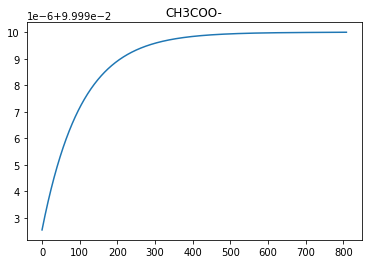
\includegraphics[width=7cm]{1.png}
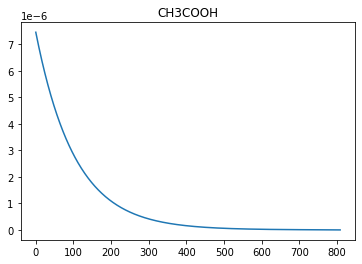
\includegraphics[width=7cm]{2.png}\\
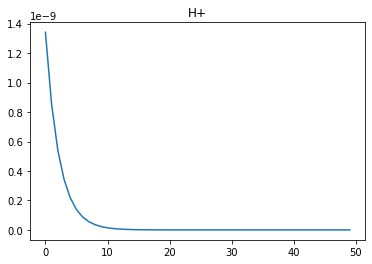
\includegraphics[width=7cm]{3.png}
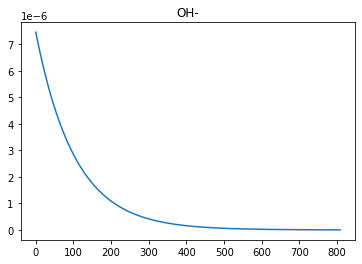
\includegraphics[width=7cm]{4.png}
\end{large}
Final activities values: 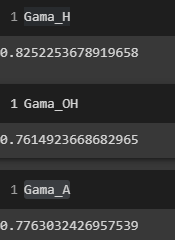
\includegraphics[width=7cm]{res.png}


\end{document}
